\documentclass[aspectratio=169,11pt]{beamer}

% Packages
\usepackage[utf8]{inputenc}
\usepackage[T1]{fontenc}
\usepackage{lmodern}
\usepackage{microtype}
\usepackage{amsmath,amssymb}
\usepackage{booktabs}
\usepackage{graphicx}
\usepackage{tikz}
\usepackage{pgfplots}
\usepackage{xcolor}
\usepackage{ragged2e}
\usepackage{colortbl}
\usepackage{array}
\usepackage{hyperref}
\usepackage{adjustbox}

\usetikzlibrary{shapes.geometric, arrows.meta, positioning, calc, backgrounds, decorations.pathreplacing, shadows, fadings}
\pgfplotsset{compat=1.18}

% --- Color Palette: Warm Professional ---
\definecolor{DeepNavy}{HTML}{2E4057}
\definecolor{Teal}{HTML}{048A81}
\definecolor{WarmOrange}{HTML}{E85D04}
\definecolor{SoftPurple}{HTML}{9D4EDD}
\definecolor{WarmGray}{HTML}{6C757D}
\definecolor{LightGray}{HTML}{E9ECEF}
\definecolor{Cream}{HTML}{FBF8F1}
\definecolor{DeepRed}{HTML}{D62828}
\definecolor{Gold}{HTML}{D4A03A}
\definecolor{SoftWhite}{HTML}{FAFAFA}

% Beamer colors
\setbeamercolor{normal text}{fg=DeepNavy, bg=SoftWhite}
\setbeamercolor{structure}{fg=DeepNavy}
\setbeamercolor{alerted text}{fg=DeepRed}
\setbeamercolor{example text}{fg=Teal}
\setbeamercolor{frametitle}{fg=DeepNavy, bg=SoftWhite}
\setbeamercolor{title}{fg=DeepNavy}
\setbeamercolor{subtitle}{fg=WarmGray}
\setbeamercolor{block title}{bg=DeepNavy, fg=SoftWhite}
\setbeamercolor{block body}{bg=LightGray, fg=DeepNavy}
\setbeamercolor{itemize item}{fg=WarmOrange}
\setbeamercolor{itemize subitem}{fg=Gold}

% Fonts
\usefonttheme{professionalfonts}
\setbeamerfont{title}{size=\huge, series=\bfseries}
\setbeamerfont{frametitle}{size=\Large, series=\bfseries}

% Strip chrome
\setbeamertemplate{navigation symbols}{}
\setbeamertemplate{headline}{}

% Minimal footline
\setbeamertemplate{footline}{%
    \hfill
    \begin{beamercolorbox}[wd=3cm,ht=2.5ex,dp=1ex,right,rightskip=0.6cm]{page number}
        \usebeamercolor[fg]{WarmGray}\scriptsize\insertframenumber
    \end{beamercolorbox}
    \vspace{0.3cm}
}

% Bullets
\setbeamertemplate{itemize item}{\footnotesize\raisebox{0.3ex}{\tikz\fill[WarmOrange] (0,0) circle (0.45ex);}}
\setbeamertemplate{itemize subitem}{\footnotesize\raisebox{0.3ex}{\tikz\fill[Gold] (0,0) circle (0.35ex);}}

% Custom commands
\newcommand{\transitionslide}[2]{%
    {\setbeamercolor{normal text}{fg=SoftWhite,bg=DeepNavy}
    \begin{frame}[plain]\vfill\begin{center}
        {\huge\bfseries\textcolor{Gold}{#1}}\\[0.6cm]
        {\large\textcolor{LightGray}{#2}}
    \end{center}\vfill\end{frame}}
}

\begin{document}

\begin{frame}
\title{Granular Instrumental Variables}
\subtitle{Estimating Aggregate Effects of Firm Shocks on Wages}
\author{Macro Lab Group Presentation}
\date{}
\titlepage
\end{frame}

\begin{frame}
\frametitle{Do shocks to superstar firms drive aggregate wage dynamics?}

\vspace{1cm}
{\Large
When a dominant employer experiences an unexpected surge in productivity, local and aggregate wages often respond.
}

\vspace{1cm}
{\Large
But how much of that response is causal, and how much is driven by common macroeconomic trends?
}

\end{frame}

\begin{frame}
\frametitle{Endogenous aggregate shocks confound the effect of large firms}

\vspace{0.5cm}
{\Large
We want to estimate the elasticity of wages to labor demand.
}

\vspace{0.5cm}
{\Large
The fundamental challenge:
}
\vspace{0.5cm}

\begin{center}
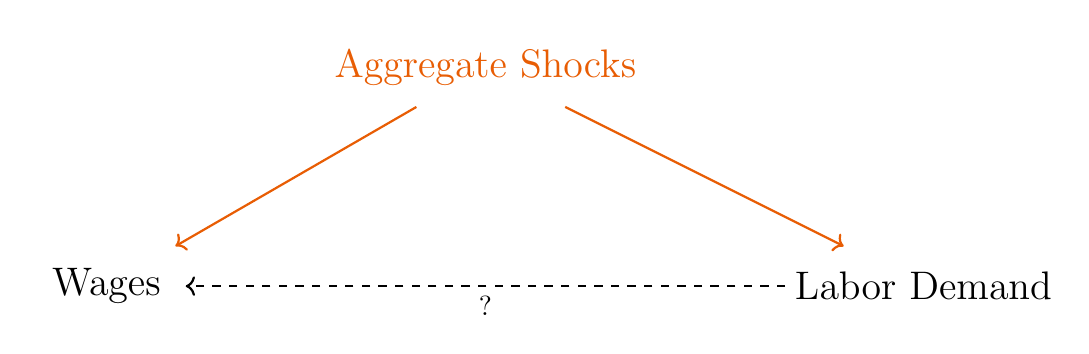
\begin{tikzpicture}[node distance=2.5cm, align=center]
  \node (common) [font=\Large, text=WarmOrange, minimum width=3cm, minimum height=1cm] {Aggregate Shocks};
  \node (wages) [below left=of common, font=\Large, minimum width=2cm, minimum height=1cm] {Wages};
  \node (demand) [below right=of common, font=\Large, minimum width=3cm, minimum height=1cm] {Labor Demand};
  
  \draw[->, thick, WarmOrange] (common) -- (wages);
  \draw[->, thick, WarmOrange] (common) -- (demand);
  \draw[->, thick, dashed] (demand) -- (wages) node[midway, below] {?};
\end{tikzpicture}
\end{center}

\end{frame}

\transitionslide{A Simple Model}{Section III.A of Gabaix and Koijen (2022)}

\begin{frame}
\frametitle{A simple model of aggregate and idiosyncratic shocks}

Consider an economy with $N$ firms and a single common factor ($\eta_t$).

\vspace{0.8cm}
The system is given by:

\vspace{0.5cm}
\begin{align}
p_t &= \psi y_{St} + \varepsilon_t \tag{38} \\[0.5cm]
y_{it} &= \phi^d p_t + \eta_t + u_{it} \tag{39}
\end{align}

\vspace{0.8cm}
Where $p_t$ is the price (or wage), $y_{St} = \sum_i S_i y_{it}$ is the size-weighted aggregate outcome, $\eta_t$ and $\varepsilon_t$ are aggregate shocks, and $u_{it}$ is the idiosyncratic shock to firm $i$.

\end{frame}

\begin{frame}
\frametitle{OLS fails because aggregate wages and common shocks are correlated}

\vspace{0.5cm}
{\Large
We cannot estimate $\psi$ and $\phi^d$ by OLS.
}

\vspace{1cm}
{\Large
Why?
}

\vspace{0.5cm}
\begin{itemize}
    \item $\varepsilon_t$ and $\eta_t$ are typically correlated.
    \item This implies that $y_{St}$ is correlated with $\varepsilon_t$ in the supply equation.
    \item And $p_t$ is correlated with $\eta_t$ in the demand equation.
\end{itemize}

\end{frame}

\begin{frame}
\frametitle{Constructing the Granular Instrumental Variable ($z_t$)}

\vspace{0.5cm}
{\Large
The GIV exploits the difference between size-weighted and equal-weighted averages.
}

\vspace{1cm}
Define the equal-weighted average outcome:
\begin{equation*}
y_{Et} = \frac{1}{N} \sum_{i=1}^N y_{it}
\end{equation*}

\vspace{0.5cm}
The GIV is the size-weighted outcome minus the equal-weighted outcome:
\begin{equation}
z_t := y_{\Gamma t} = y_{St} - y_{Et} \tag{40}
\end{equation}

\end{frame}

\begin{frame}
\frametitle{The GIV isolates purely idiosyncratic firm shocks}

\vspace{0.5cm}
Substitute the demand equation into the aggregate definitions:
\begin{align}
y_{St} &= \phi^d p_t + \eta_t + u_{St} \notag \\
y_{Et} &= \phi^d p_t + \eta_t + u_{Et} \tag{41}
\end{align}

\vspace{0.5cm}
The common components ($\phi^d p_t + \eta_t$) difference out:
\begin{equation}
z_t = u_{\Gamma t} = u_{St} - u_{Et} \tag{42}
\end{equation}

\vspace{0.5cm}
{\Large
$z_t$ is made \emph{only} of idiosyncratic shocks.
}

\end{frame}

\begin{frame}
\frametitle{The GIV yields both supply and demand elasticities}

\vspace{0.5cm}
By exogeneity, $\mathbb{E}[u_t \varepsilon_t] = 0 \implies \mathbb{E}[z_t \varepsilon_t] = 0$.

\vspace{0.5cm}
Using the supply equation (38), $\mathbb{E}[(p_t - \psi y_{St}) z_t] = 0$:
\begin{equation*}
\psi = \frac{\mathbb{E}[p_t z_t]}{\mathbb{E}[y_{St} z_t]}
\end{equation*}

\vspace{0.5cm}
Using the equal-weighted demand equation, $\mathbb{E}[(y_{Et} - \phi^d p_t) z_t] = 0$:
\begin{equation*}
\phi^d = \frac{\mathbb{E}[y_{Et} z_t]}{\mathbb{E}[p_t z_t]}
\end{equation*}

\end{frame}



\begin{frame}
\frametitle{Identifying wage spillovers from superstar firms}

\vspace{0.5cm}
{\Large
How do we apply GIVs to labor markets?
}

\vspace{1cm}
\begin{itemize}
    \item \textbf{The granular shock:} Use idiosyncratic productivity or demand shocks of the largest employers in a region.
    \item \textbf{The instrument:} The GIV ($z_t$) aggregates these large-firm idiosyncratic shocks.
    \item \textbf{The estimation:} Instrument local or aggregate wage changes ($p_t$) using the GIV to estimate the causal impact of labor demand on wages ($\psi$).
\end{itemize}

\end{frame}

\begin{frame}
\frametitle{GIV precision relies on concentrated labor markets and volatile micro-shocks}

\vspace{0.5cm}
{\Large
For the instrument to be strong, we need:
}

\vspace{1cm}
\begin{enumerate}
    \item \textbf{A large excess Herfindahl index ($h$):} A few superstar firms must account for a substantial fraction of total employment.
    \vspace{0.5cm}
    \item \textbf{Volatile idiosyncratic shocks ($\sigma_u$):} Firm-specific shocks must be large relative to aggregate macroeconomic volatility ($\sigma_\varepsilon$).
\end{enumerate}

\end{frame}

\end{document}